\title{Study Guide for Midterm 2}
\author{Dr. Jordan Hanson - Whittier College Dept. of Physics and Astronomy}
\date{\today}
\documentclass[10pt]{article}
\usepackage[a4paper, total={18cm, 27cm}]{geometry}
\usepackage{outlines}
\usepackage{graphicx}
\begin{document}
\maketitle

\section{Chapter 5 - Combinatorial Logic Analysis}
\label{sec:comb}

\begin{figure}[ht]
\centering
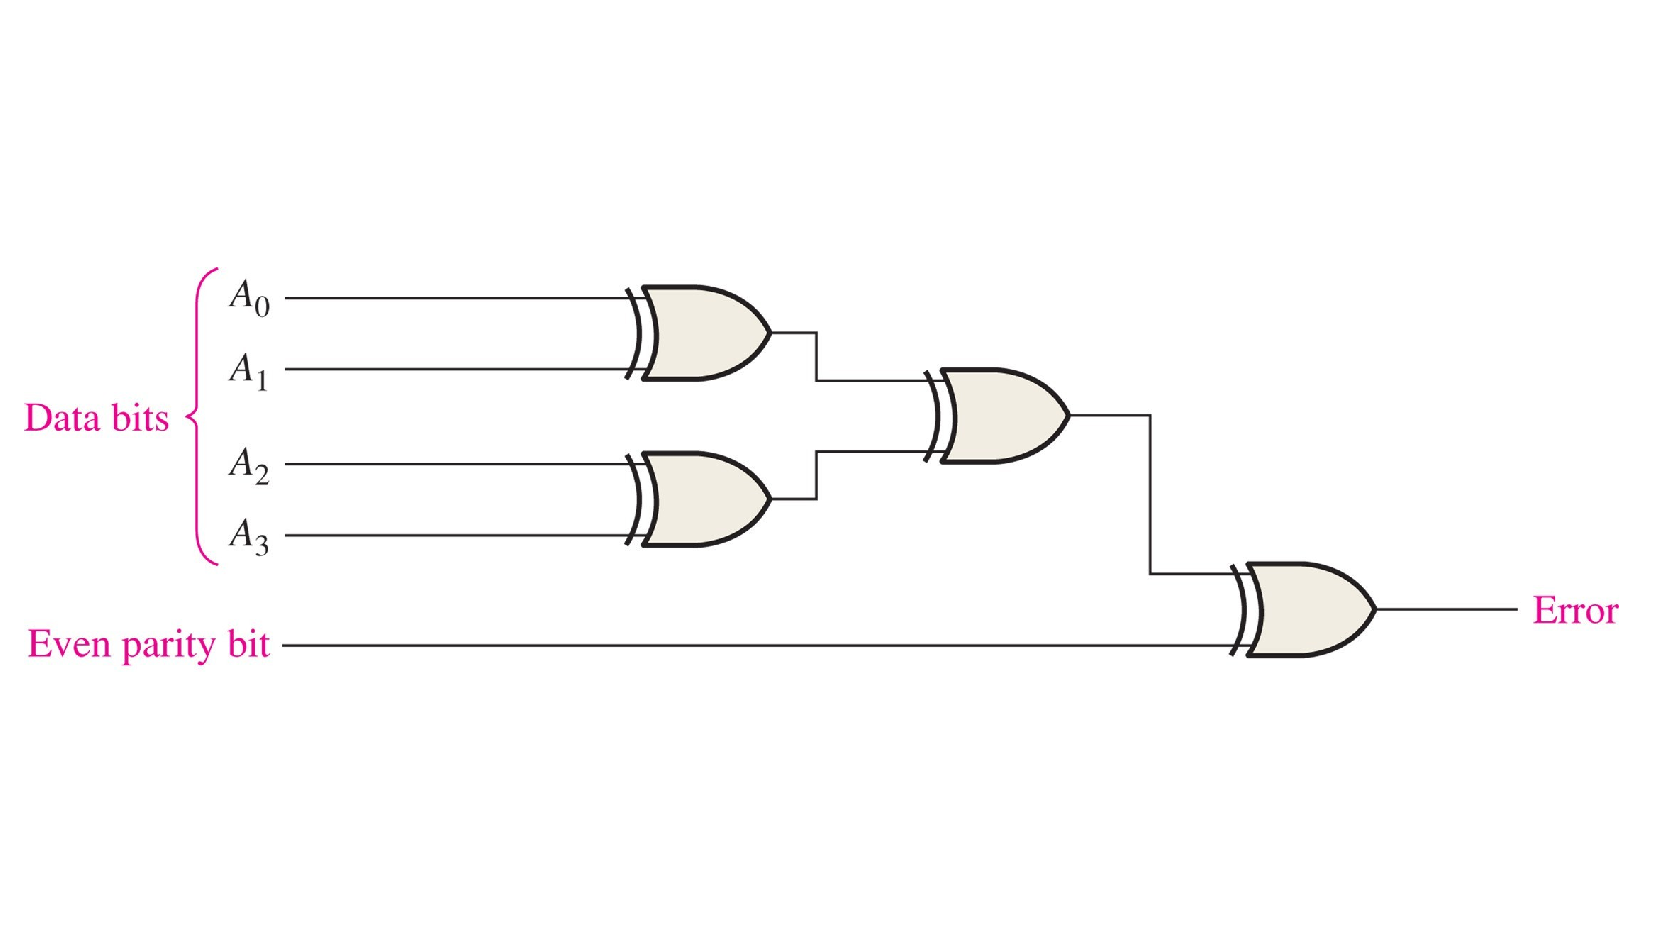
\includegraphics[width=0.45\textwidth,trim=0cm 4cm 0cm 4cm,clip=true]{figures/parityCheck.pdf} \hspace{0.25cm}
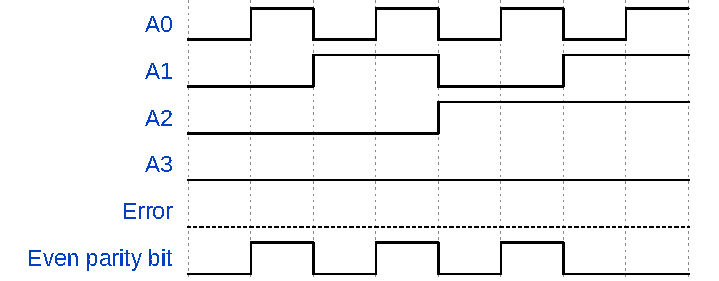
\includegraphics[width=0.4\textwidth]{figures/timingExample9.pdf}
\caption{\label{fig:par} (Left) A circuit involving several XOR gates. (Right) An example timing diagram for the circuit at left.}
\end{figure}

\begin{enumerate}
\item Consider Fig. \ref{fig:par}.  (a) Generate the truth table for the output of the first three XOR gates, for all possible values of the 4-bit binar	y input.  What does this output represent numerically about the input $\vec{A}$? (b) Fill in the Error bit stream in Fig. \ref{fig:par}. \\ \vspace{1cm}
\item In Fig. \ref{fig:gates1}, (a) simplify the circuit via the Karnaugh map. (b) For the resulting domain-2 logic function, connect $A0$ and $A1$ from Fig. \ref{sec:comb} (right) as inputs and produce the timing diagram assuming the same even parity bit stream.\\ \vspace{2cm}
\end{enumerate}

\begin{figure}[hb]
\centering
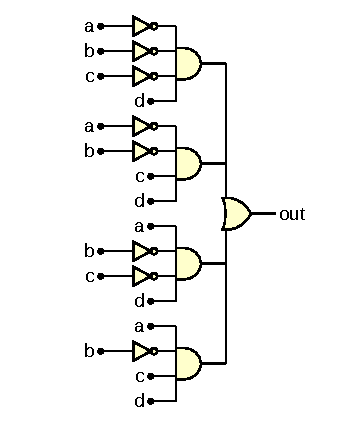
\includegraphics[width=0.3\textwidth]{figures/gateExample6.pdf}
\caption{\label{fig:gates1} A domain-4 logic function.}
\end{figure}

\clearpage

\section{Chapter 6 - Functions of Combinational Logic}
\label{sec:comb2}

\begin{figure}[ht]
\centering
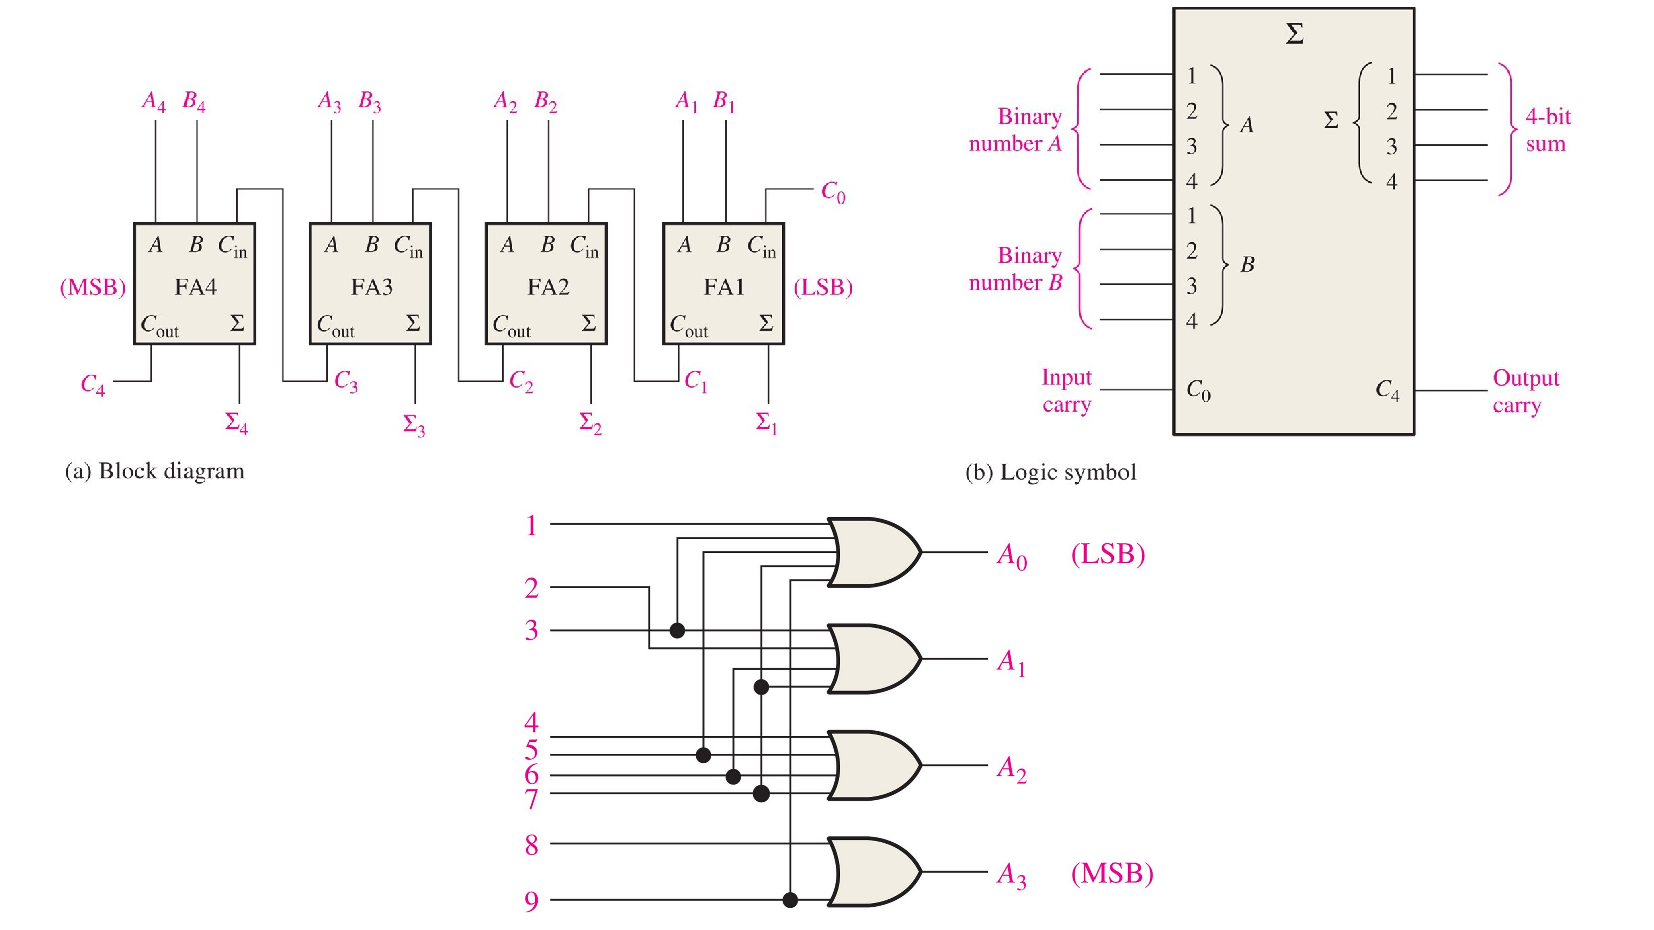
\includegraphics[width=0.6\textwidth]{figures/adderEncoder.pdf}
\caption{\label{fig:encadd} A 4-bit ripple carry adder (with logic symbol), and a 9-digit (zero ommitted) encoder.}
\end{figure}

\begin{enumerate}
\item Consider Fig. \ref{fig:encadd}.  (a) Design a circuit below that adds two numbers in binary corresponding to outputs from two separate encoders. (b) Demonstrate how your design would add 1 and 9.  (c) Add a separate input line with XNOR gates that switches the system to subtraction in 2's complement form. \\ \vspace{3cm}
\item Using the basic logic in Fig. \ref{fig:2bit}, plus inverters, (a) create a circuit that compares the \textit{magnitude} of two 2-bit binary numbers.  Assume that one or both of the numbers is a negative one, and that if a number is negative it is in \textit{1's complement form.} \\ \vspace{3cm}
\item For the first four binary numbers (0, 1, 2, 3) show that the logic in Fig. \ref{fig:2bit} (right) converts binary to gray code.
\end{enumerate}

\begin{figure}[hb]
\centering
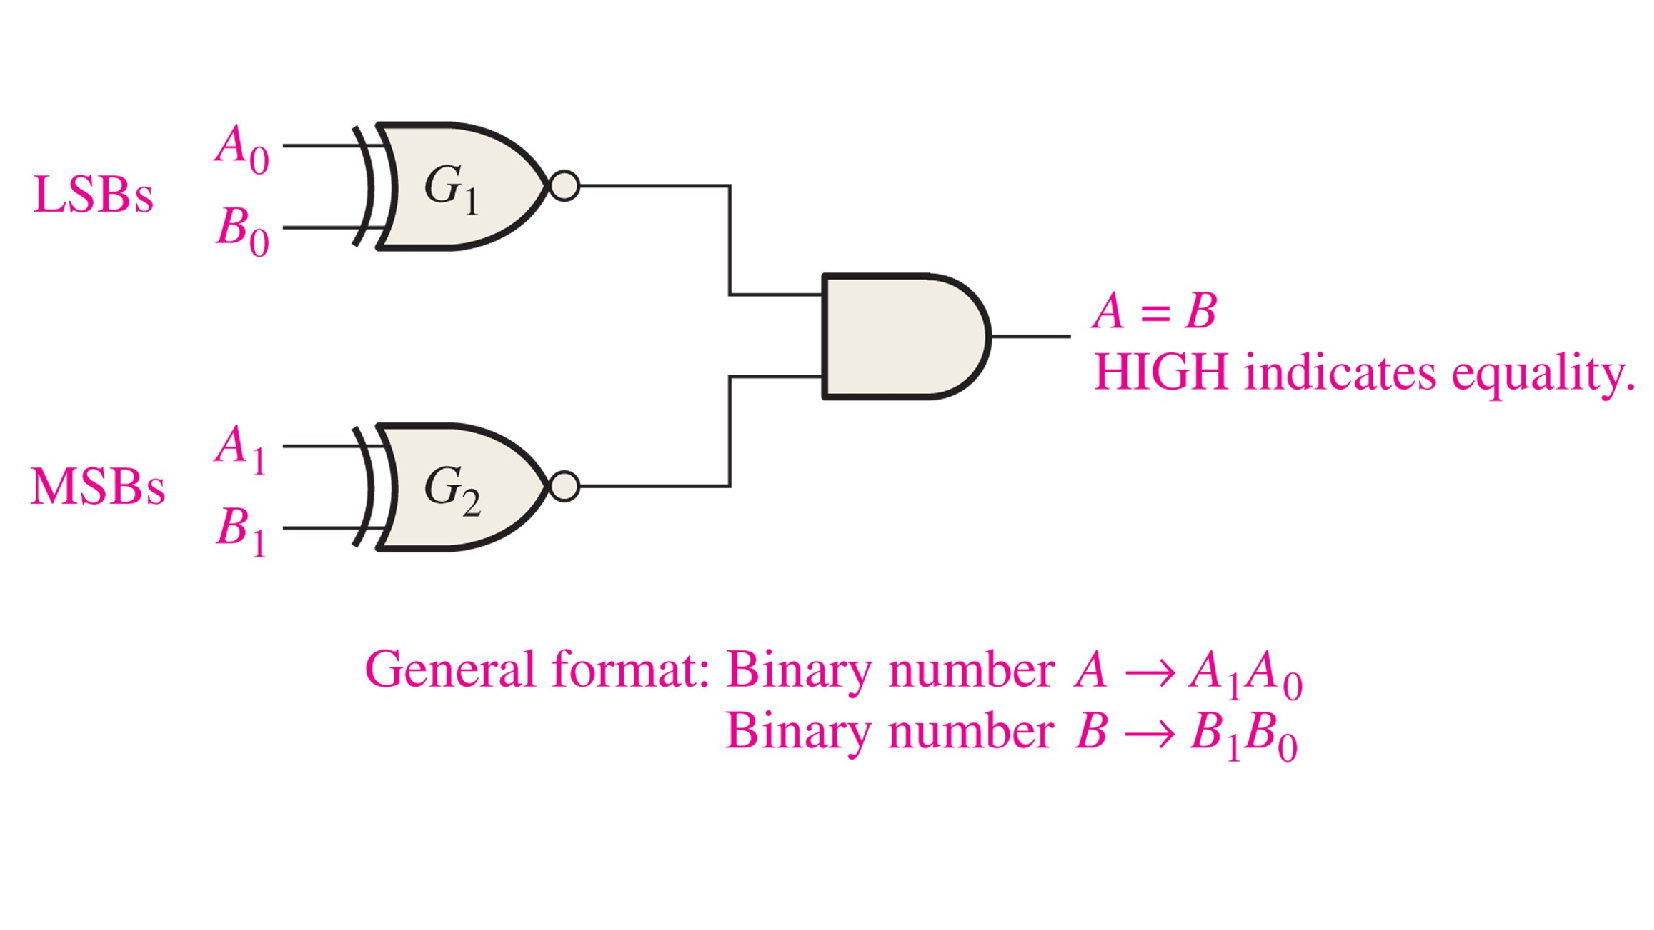
\includegraphics[width=0.4\textwidth]{figures/2bitcomparator.pdf} \hspace{0.25cm}
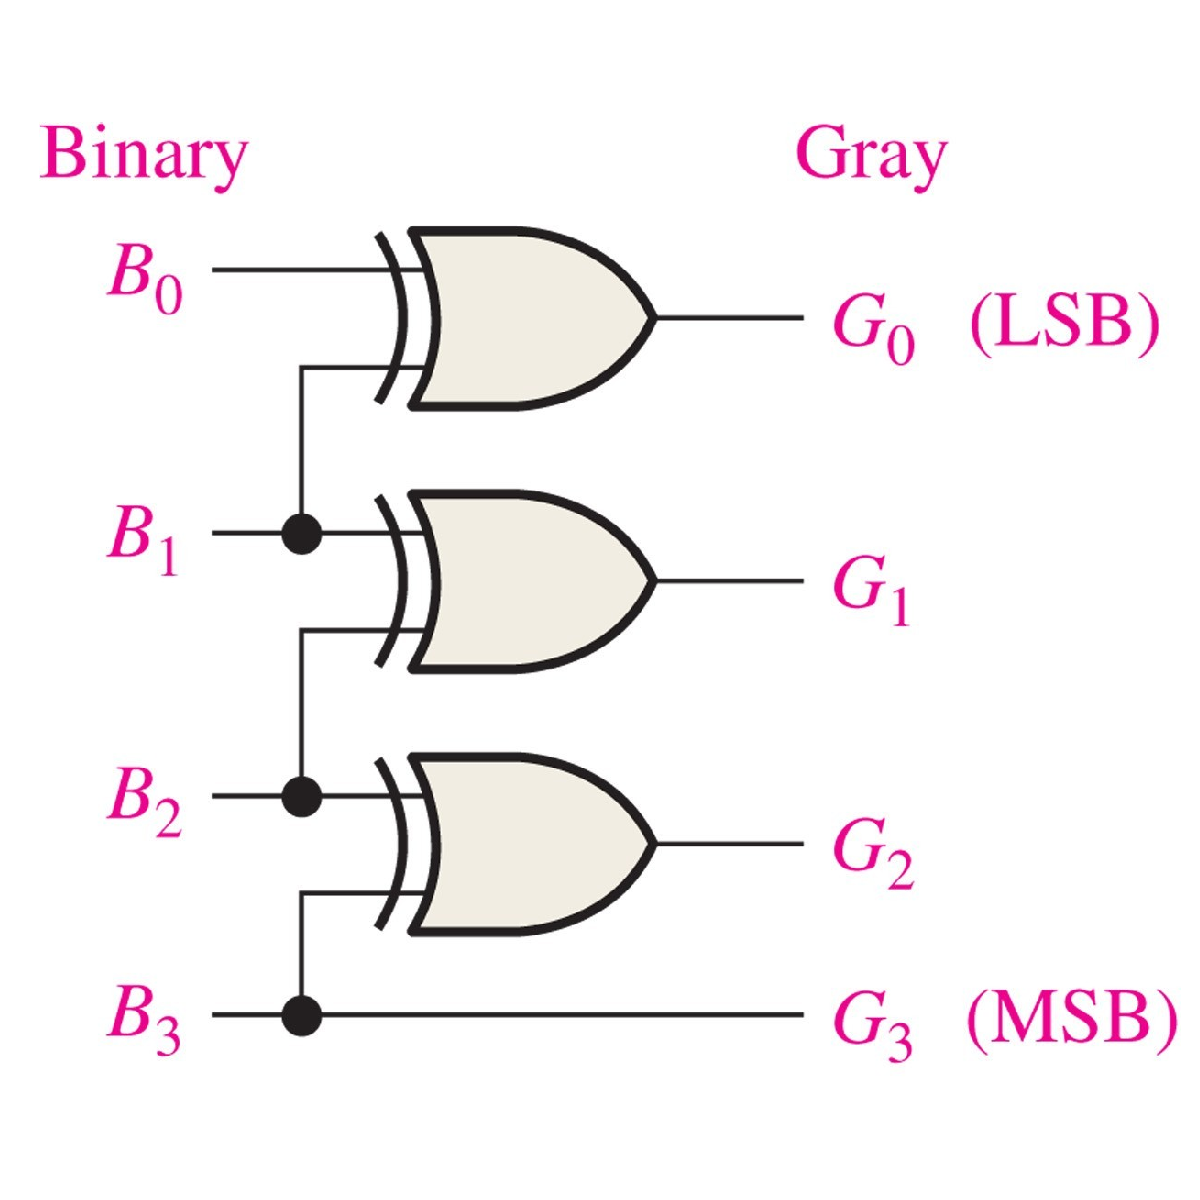
\includegraphics[width=0.25\textwidth]{figures/binaryGray.pdf}
\caption{\label{fig:2bit} (Left) This is how a 2-bit comparator works. (Right) A binary to gray code converter.}
\end{figure}

\clearpage

\section{Chapter 7 - Latches, Flip-flops, and Timers}
\label{sec:latch}

\begin{figure}[ht]
\centering
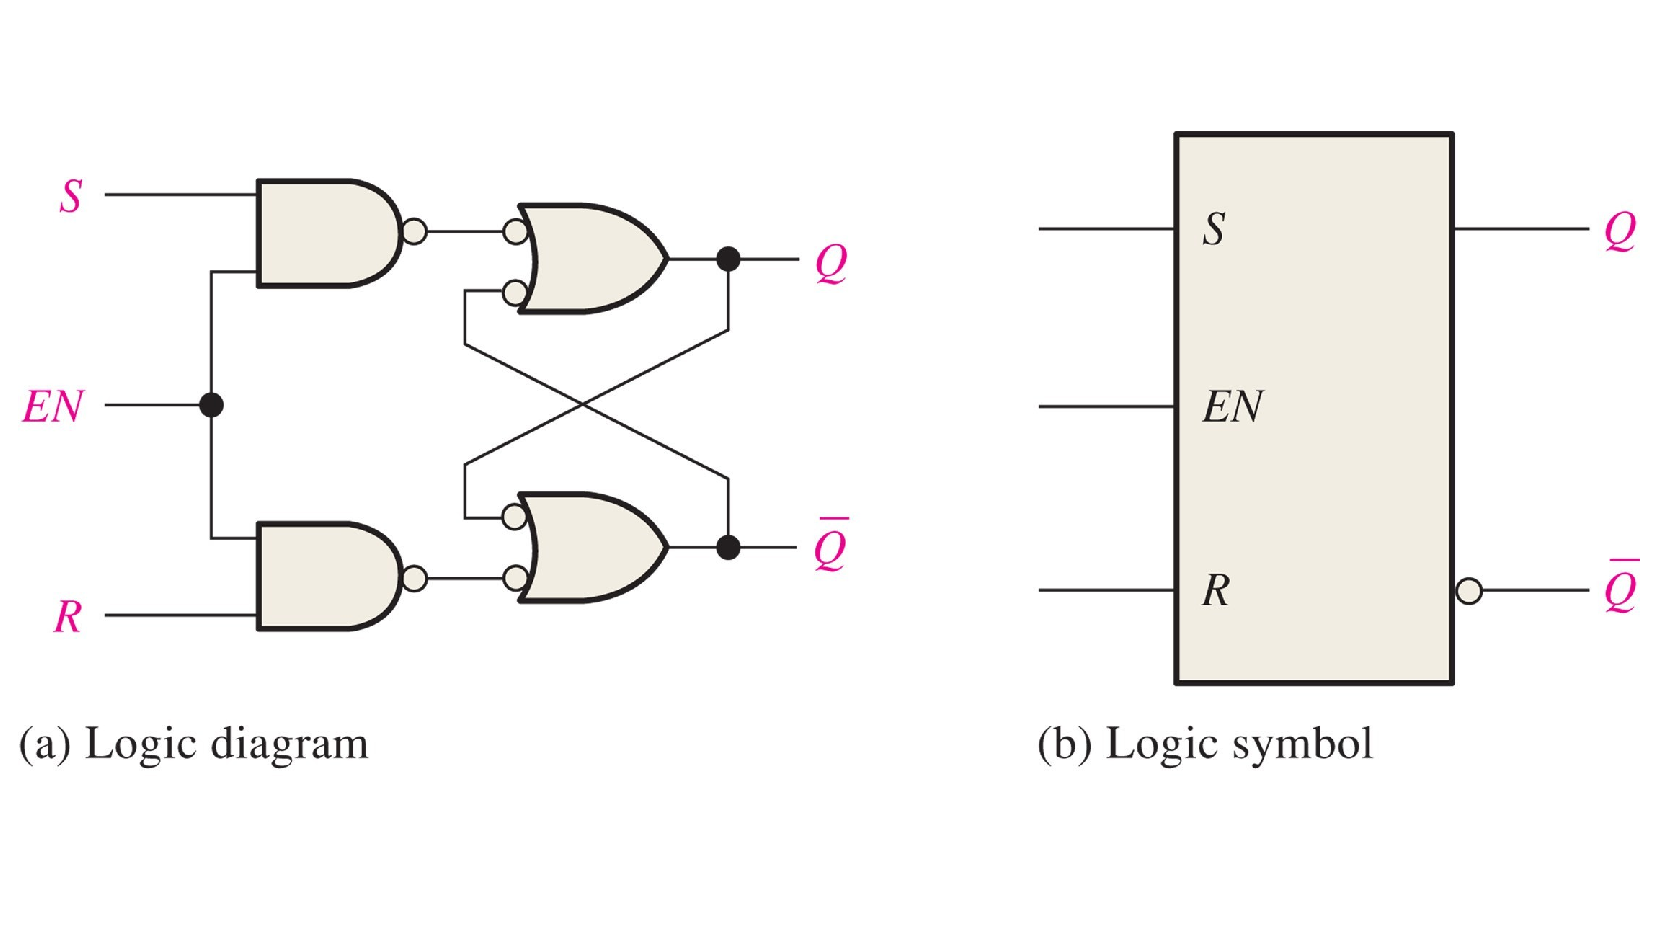
\includegraphics[width=0.5\textwidth]{figures/enSRLatch.pdf} \hspace{0.5cm}
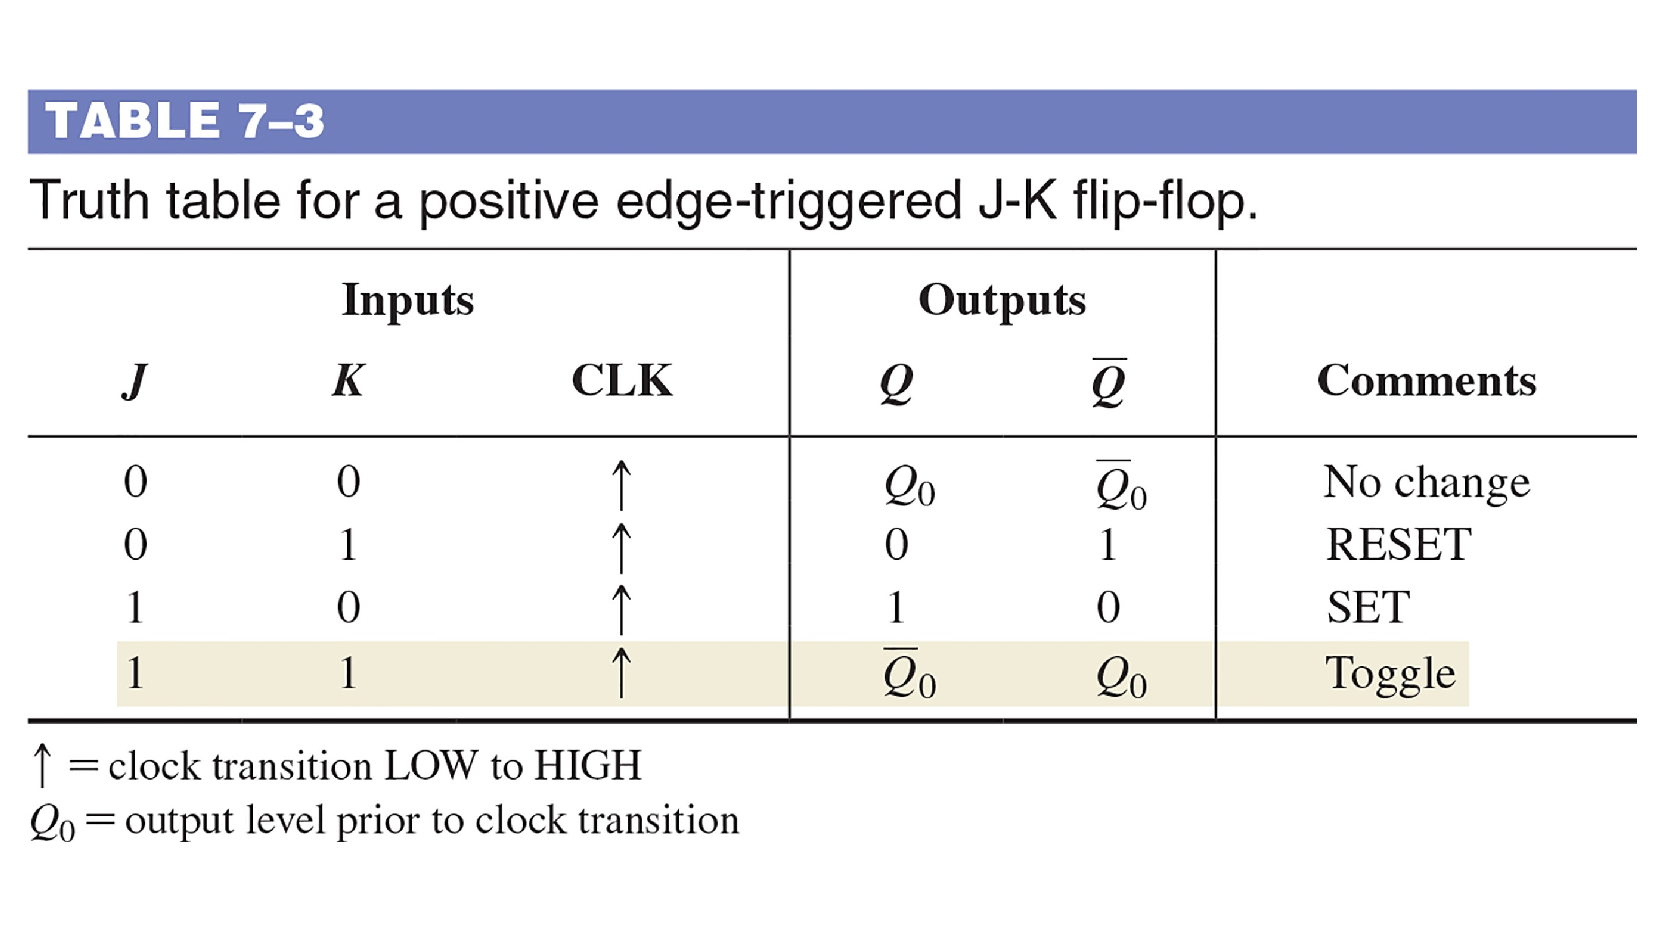
\includegraphics[width=0.5\textwidth]{figures/jkFlopTT.pdf}
\caption{\label{fig:latch} (Top) The gate-enabled SR latch. (Bottom) The truth table for the JK flip-flop.}
\end{figure}

\begin{enumerate}
\item Using the logic for the gate-enabled SR latch in Fig. \ref{fig:latch} (top), develop a system that (a) activates a green LED when the circuit is enabled and in SET mode, (b) a yellow LED switch when the circuit is enabled and in RESET mode, and (c) a red LED when the circuit is not enabled. \\ \vspace{2cm}
\item The truth table for a positive clock-edge JK flip-flop is shown in Fig. \ref{fig:latch} (bottom).  Use such a device to design a circuit below that (a) powers two LEDs, and toggles between two states: one in which one LED is activated, and another in which the opposite LED is activated. The lights should switch on positive edges of the clock.  (b) Add logic that holds LED1 on, and LED2 off, regardless of the outputs of the JK flip-flop (the equivalent of \textit{preset} and \textit{clear} functions of JK flip-flops).
\end{enumerate}

\end{document}